\documentclass{beamer} 

\mode<presentation> {
    \usetheme{ARAMIS}
}

\usepackage[english]{babel}
\usepackage[utf8]{inputenc}

\usepackage{ragged2e}
\usepackage{amsmath,amsthm, amssymb, latexsym}
\usefonttheme[onlymath]{serif}


%%%%%%%%%%%%%%%%
%%% LISTINGS %%%
%%%%%%%%%%%%%%%%
\usepackage{listings}
\definecolor{colString}{rgb}{0.6,0.1,0.1} 
\definecolor{Green}{rgb}{0.1,0.5,0.1}
\lstset{%configuration de listings 
	float=hbp,% 
	language={C},%
	morekeywords={assert, then},%
	basicstyle=\ttfamily\protect\fontsize{26pt}{26pt}\protect\selectfont, % 
	backgroundcolor=\color{white},%
	identifierstyle=\color{black}, % 
	keywordstyle=\color{blue}, % 
	stringstyle=\color{colString}, % 
	commentstyle=\color{Green}, % 
	columns=flexible, % 
	keepspaces=true,  % keeps spaces in text, useful for keeping indentation of code
	escapeinside={\%*}{*)},%
	tabsize=4, % 
	frame=l, % 
	frameround=tttt, % 
	extendedchars=true, % 
	showspaces=false, % 
	showstringspaces=false, % 
	%numbers=left, % 
	numbersep=5pt,
    numberstyle=\protect\fontsize{16pt}{16pt}\protect\selectfont\ttfamily\color{black}, % 
	breaklines=true, % 
	xleftmargin=40pt, %
	breakautoindent=true, % 
	captionpos=b,% 
    framesep=10pt,
} 


\usepackage[orientation=portrait,size=a0,scale=1.4,debug]{beamerposter}           % e.g. for DIN-A0 poster
%\usepackage[orientation=portrait,size=a1,scale=1.4,grid,debug]{beamerposter}     % e.g. for DIN-A1 poster, with optional grid and debug output
%\usepackage[size=custom,width=200,height=120,scale=2,debug]{beamerposter}        % e.g. for custom size poster
%\usepackage[orientation=portrait,size=a0,scale=1.0,printer=rwth-glossy-uv.df]{beamerposter}     % e.g. for DIN-A0 poster with rwth-glossy-uv printer check
% ...
%
\usepackage{tcolorbox}
\tcbset{%
    noparskip,
    colback=white, %background color of the box
    colframe=normalTitleBlockColor, %color of frame and title background
    coltext=black, %color of body text
    coltitle=black, %color of title text 
    %fonttitle=\bfseries,
    %valign upper=center,
    %boxsep=2mm,
    boxrule=1.5mm,
    alerted/.style={coltitle=red, 
                     colframe=gray!40},
    example/.style={coltitle=black, 
                     colframe=green!20,             
                     colback=green!5},
    }

\usepackage{tikz}
\usetikzlibrary{arrows,snakes,backgrounds,patterns,matrix,shapes,fit,calc,shadows,plotmarks,intersections,shapes.geometric}


\beamertemplatenavigationsymbolsempty

\usepackage{xspace}
\newcommand{\TODO}{{\color{red}\bf [TODO]}}
\newcommand{\cybersec}{cybersecurity\xspace}
\newcommand{\Cybersec}{Cybersecurity\xspace}
\newcommand{\aramis}{Aramis\xspace}
\newcommand{\proverif}{ProVerif\xspace}
\newcommand{\DiH}{Diffie-Hellman\xspace}
\newcommand{\XOR}{Exclusive-Or\xspace}
\newcommand{\modbus}{MODBUS\xspace}
\newcommand{\opcua}{OPC-UA\xspace}
\newcommand{\eg}{e.g.:\xspace}
\newcommand{\ftpauth}{FTP$_{Auth}$\xspace}
\newcommand{\opcuasignenc}{OPC-UA$_{SignEnc}$\xspace}

\usepackage{pifont}% http://ctan.org/pkg/pifont
\newcommand{\cmark}{{\color{green}\ding{51}}}%
\newcommand{\xmark}{}%{\color{red}\ding{55}}}%
\newcommand{\omark}{{\color{orange}$\mathcal{O}$}}%

\graphicspath{{assets/}}
\makeatletter
    \def\input@path{{assets/}}
\makeatother

\title{Formal Analysis and Smart-Fuzzing of Industrial Systems}
\author{Maxime Puys, Marie-Laure Potet and Jean-Louis Roch}
\institute{VERIMAG, University of Grenoble Alpes, France\\{\texttt Firstname.Name@imag.fr}}
\date{}

\begin{document}

\begin{frame}[fragile]{}
    \begin{columns}[T]
        \begin{column}{.49\textwidth}
            \begin{tcolorbox}[adjusted title={\centering\large Industrial Systems}]
                \vspace{.25em}
                \begin{itemize}
                    \item Supervisory Control And Data Acquisition.
                \end{itemize}
                \centering
                \begin{columns}
                    \begin{column}{.3\textwidth}
                        \centering
                        \resizebox{\textwidth}{!}{
                            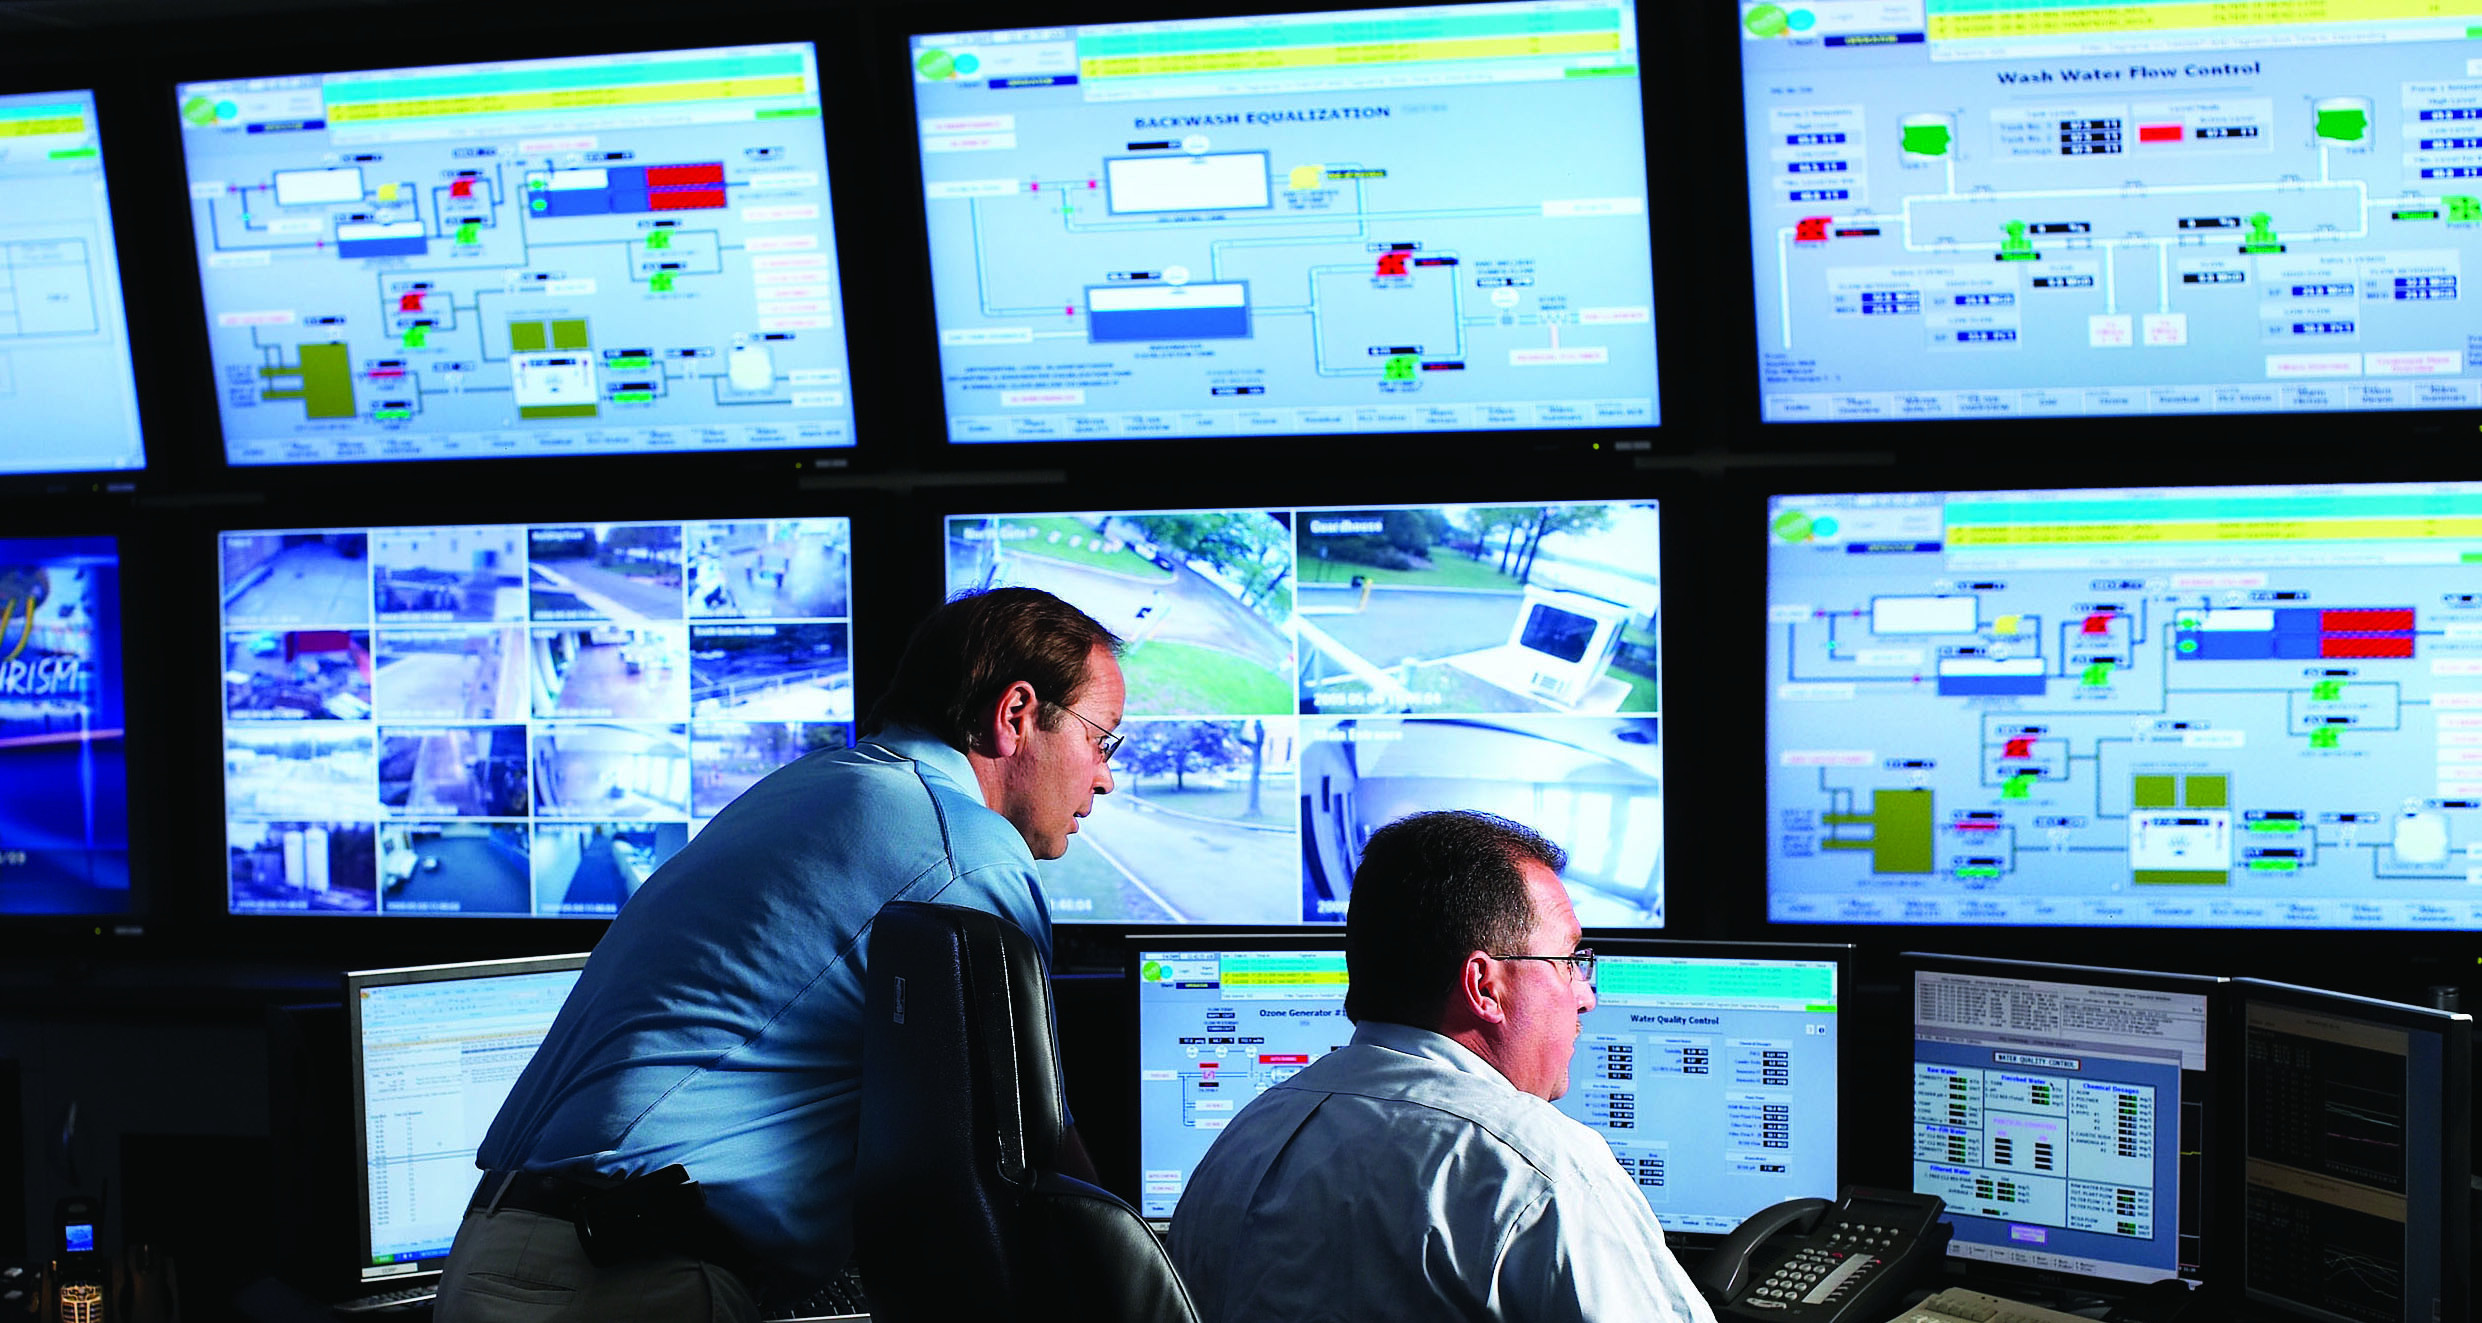
\includegraphics{scada}
                        }
                    \end{column}
                    \begin{column}{.3\textwidth}
                        \centering
                        \resizebox{.89\textwidth}{!}{
                            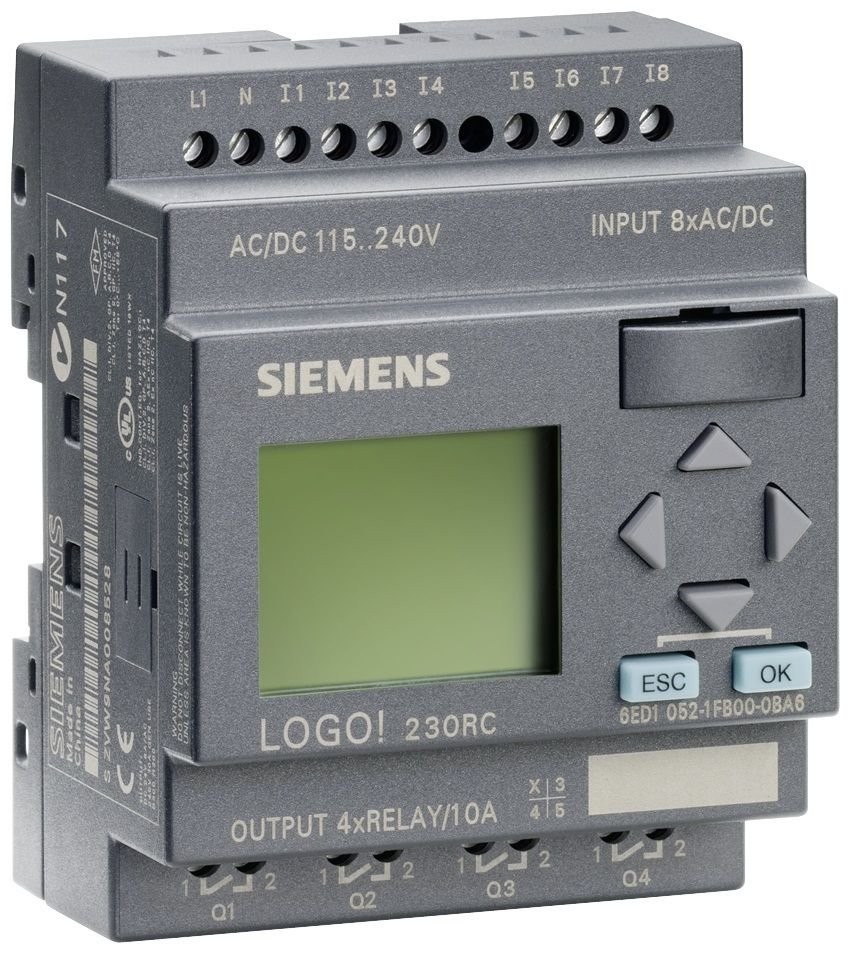
\includegraphics{plc}
                        }
                    \end{column}
                    \begin{column}{.3\textwidth}
                        \centering
                        \resizebox{\textwidth}{!}{
                            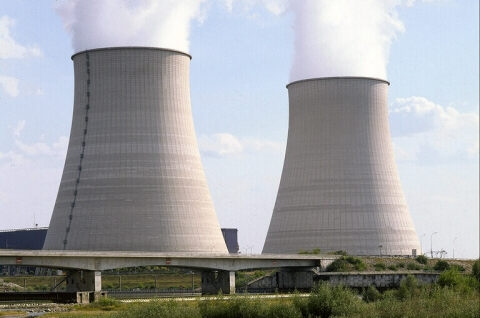
\includegraphics{plant}
                        }
                    \end{column}
                \end{columns}
                \begin{itemize}
                    \item Increasing number of attacks showed in the medias since Stuxnet.
                    \item Becoming a priority for government agencies.
                    \begin{itemize}
                        \item Laws to ensure the security of OIVs ({\em Loi de Programmation Militaire, Livre blanc sur la défense et la sécurité nationale}).
                        \item Publications from ANSSI, DGA, ...
                    \end{itemize}
                \end{itemize}
            \end{tcolorbox}
        \end{column}
        %\hfill
        \begin{column}{.49\textwidth}
            \begin{tcolorbox}[adjusted title={\centering\large Security concepts}]
                \vspace{.25em}
                \begin{itemize}
                    \item Safety = Protection against identified/natural difficulties.
                    \begin{itemize}
                        \item Historic industrial concern.
                    \end{itemize}
                    \item \Cybersec = Protection against malicious adversaries.
                    \begin{itemize}
                        \item Often called Security.
                    \end{itemize}
                \end{itemize}

                \vspace{-.6em}
                \begin{columns}[c]
                    \begin{column}{.49\textwidth}
                        \begin{figure}[htb]
                            \resizebox{1.1\columnwidth}{!}{
                                \def\rectangle{(-1.5,-4.5) rectangle (12,5.25)}
\def\secondcircle{(0:15.75) ellipse (6 and 4.5)}
\def\thridcircle{(0:-5.25) ellipse (6 and 4.5)}
\def\fourthcircle{(0:5.25) ellipse (6.75 and 3)}

\begin{tikzpicture}
    \draw \rectangle node at (5.25,4) {Industrial systems};
    \draw \secondcircle node {\Cybersec};
    \draw \thridcircle node {Safety};
    \draw \fourthcircle node [align=center]{Industrial \\ systems \\ \cybersec};
    \begin{scope}[fill opacity=0.25]
        \fill[blue]   \rectangle;
        \fill[red]    \secondcircle;
        \fill[green]  \thridcircle;
        \fill[yellow] \fourthcircle;
    \end{scope}
\end{tikzpicture}

                            }
                            \vspace{-1.7cm}
                            \caption{Relations among security concepts}
                        \end{figure}
                    \end{column}
                    \begin{column}{.49\textwidth}
                        \begin{figure}[htb]
                            \vspace{-1em}
                            \resizebox{1.1\columnwidth}{!}{
                                \begin{tikzpicture}[
    myarrow/.style={
        draw=black,solid,line width=2mm, postaction={-triangle 90,thin,draw,shorten >=-1mm}
}]
    %\draw[->, very thick] (0,0) -- (0,-1) -- (1,-1.5) -- (1,-2.5) -- (0,-3);
    \path[myarrow, gray] (0,5) -- (0,1);
    \path[myarrow] (1,5) -- (1,1);
    \draw node [align=center] at (.5,0) {\tiny Historical};
    \draw node [align=center] at (.5,-.6) {\tiny Approach};

    \draw[dashed] (2,-1) -- (2,6);

    \fill[gray] (3.4,1) rectangle (3.5,5);
    \fill[black] (3.5,1) rectangle (3.6,5);
    \draw (3.35,1) -- (3.65,1) -- (3.5,.85) -- cycle;
    \draw node [align=center] at (3.5,0) {\tiny Unified};
    \draw node [align=center] at (3.5,-.6) {\tiny Approach};

    \draw[red] (2,-1) -- (5,6);
    \draw[red] (5,-1) -- (2,6);

    \draw[dashed] (5,-1) -- (5,6);
    
    \path[myarrow, gray] (6,5) -- (6,1);
    \path[myarrow] (7,5) -- (7,1);
    \draw[->,thick] (6.85,5) -- (6.15,4.1);
    \draw[->,thick] (6.15,4) -- (6.85,3.1);
    \draw[->,thick] (6.85,3) -- (6.15,2.1);
    \draw[->,thick] (6.15,2) -- (6.85,1.1);
    \draw node [align=center] at (6.5,0) {\tiny Coordinated};
    \draw node [align=center] at (6.5,-.6) {\tiny Approach};

    \draw[dashed] (8,-1) -- (8,6);
    
    \path[myarrow, gray] (9,5) -- (9,4) -- (9.5,3.5) -- (9.5,2.5) -- (9,2) -- (9,1);
    \path[myarrow] (10.2,5) -- (10.2,4) -- (9.7,3.5) -- (9.7,2.5) -- (10.2,2) -- (10.2,1);
    \draw node [align=center] at (9.6,0) {\tiny Integrated};
    \draw node [align=center] at (9.6,-.6) {\tiny Approach};
\end{tikzpicture}

                            }
                            \vspace{-2.5cm}
                            \caption{Relations among security concepts}
                            \vspace{.75em}
                        \end{figure}
                    \end{column}
                \end{columns}
            \end{tcolorbox}
        \end{column}
    \end{columns}
    \vspace{.25em}
    \begin{tcolorbox}[adjusted title={\centering\large Formal Analysis of Industrial Protocols}]
        \vspace{.5em}
        \begin{columns}[T]
            \begin{column}{.35\textwidth}
                \begin{tcolorbox}[
                colback=white, %background color of the box
                colframe=normalTitleBlockColor, %color of frame and title background
                colframe=gray!20, %color of frame and title background
                boxrule=1mm,
                coltext=black, %color of body text
                coltitle=black, %color of title text
                bottom=2mm,
                equal height group=B,
                valign = center,
                adjusted title={\large Objectives}]
                    \vspace{.5em}
                    \begin{itemize}
                        \item Modeling in the {\bf $\pi$-calculus language} of:
                        \begin{itemize}
                            \item Industrial protocols such as \modbus and \opcua.
                            \item Security properties of secrecy and authentication.
                        \end{itemize}
                    \vspace{.5em}
                        \item Analyze by the {\bf \proverif} prover:
                        \begin{itemize}
                            \item Intruder follows decisional {\bf Dolev-Yao} model.
                            \item Results: either a formal proof of security or an attack trace.
                        \end{itemize}
                    \vspace{.5em}
                        \item Literature involves analysis of e-voting, e-cash, e-reputation, e-exams, etc.
                    \vspace{.5em}
                    \item Industrial systems requires more complex properties: {\bf integrity} and {\bf availability}.
                    \end{itemize}
                \end{tcolorbox}
            \end{column}
            \begin{column}{.65\textwidth}
                \begin{tcolorbox}[
                colback=white, %background color of the box
                colframe=normalTitleBlockColor, %color of frame and title background
                colframe=gray!20, %color of frame and title background
                boxrule=1mm,
                coltext=black, %color of body text
                coltitle=black, %color of title text
                bottom=2mm,
                equal height group=B,
                valign = center,
                adjusted title={\large Approach}]
                    \begin{columns}[c]
                        \begin{column}{.45\textwidth}
                            \begin{figure}[htb]
                                \resizebox{\textwidth}{!}{
                                    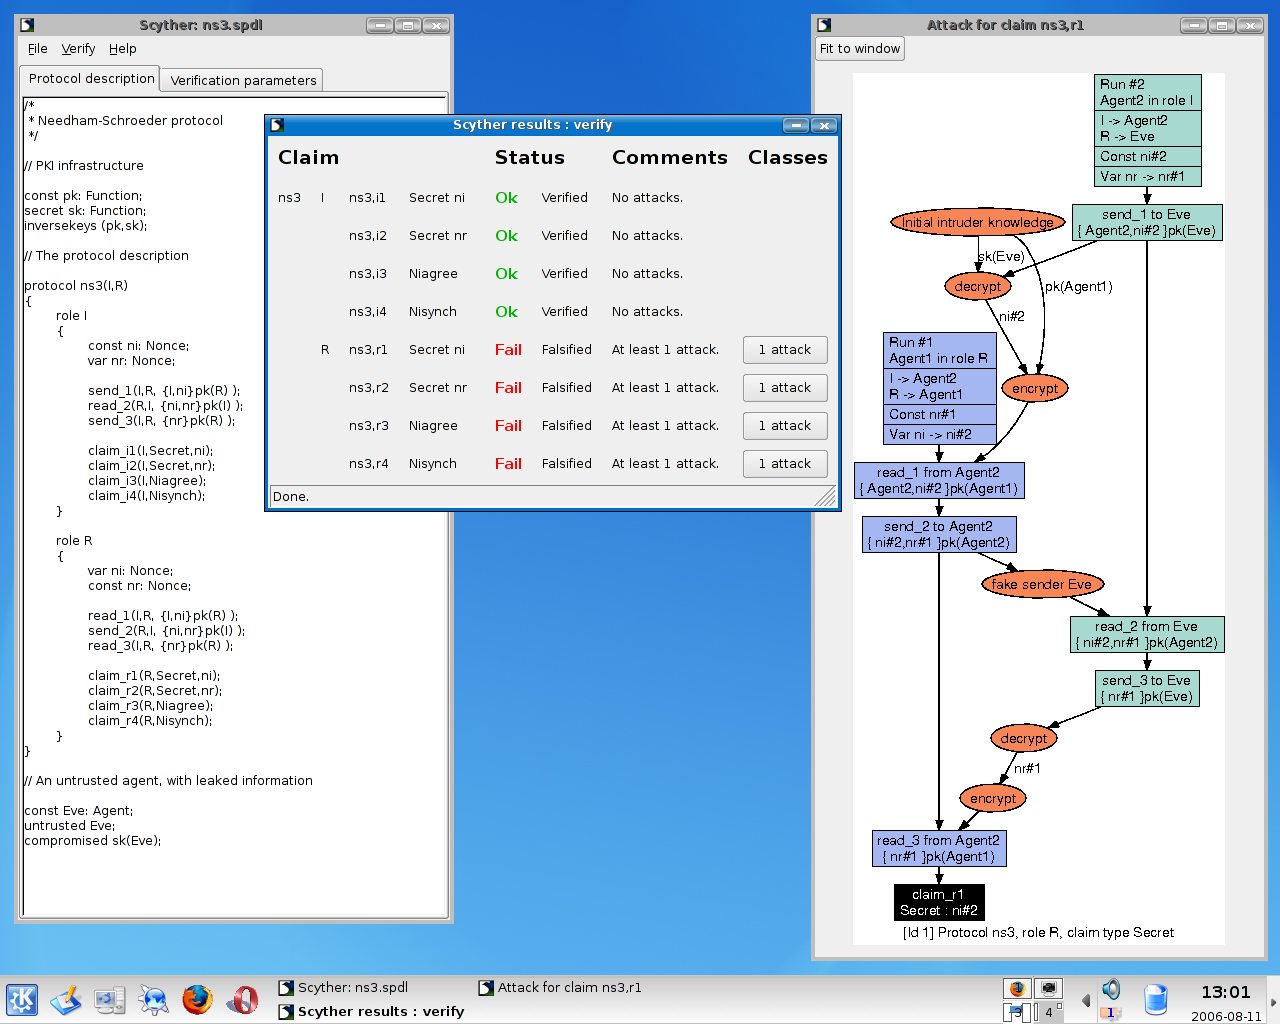
\includegraphics{scyther-linux}
                                }
                                \vspace{-1.25em}
                                \caption{The Scyther tool}
                            \end{figure}
                        \end{column}
                        \begin{column}{.55\textwidth}
                            \begin{figure}[htb]
                                \resizebox{\textwidth}{!}{
                                    \includegraphics{opcua}
                                }
                                \vspace{-1.25em}
                                \caption{\opcua OpenSecureChannel sub-protocol}
                            \end{figure}
                        \end{column}
                    \end{columns}
                \end{tcolorbox}
            \end{column}
        \end{columns}
    \end{tcolorbox}
    \vspace{.25em}
    \begin{tcolorbox}[adjusted title={\centering\large Smart-Fuzzing of Industrial Systems}]
        \vspace{.5em}
        \begin{columns}[T]
            \begin{column}{.35\textwidth}
                \begin{tcolorbox}[
                colback=white, %background color of the box
                colframe=normalTitleBlockColor, %color of frame and title background
                colframe=gray!20, %color of frame and title background
                boxrule=1mm,
                coltext=black, %color of body text
                coltitle=black, %color of title text
                bottom=2mm,
                equal height group=C,
                valign = center,
                adjusted title={\large Objectives}]
                    \vspace{.5em}
                    \begin{itemize}
                        \item Modeling in the {\bf CSP language} of:
                        \begin{itemize}
                            \item Industrial infrastructures (components, network links and communication protocols),
                            \item Threats (in terms of position, capacities and objectives),
                            \item Security objectives (\eg "This services needs authentication.") and safety properties (\eg "Electricity consumption always remains lower than production").
                        \end{itemize}
                        \item Automaticaly produce abstract attack scenarios that an adversary should follow to achieve one of his objective using the {\bf FDR3 model-checker}.
                        \item Convert attack scenarios to real network packets with the {\bf Scapy} python package to verify and quantify their plausibility.
                    \end{itemize}
                \end{tcolorbox}
            \end{column}
            \begin{column}{.65\textwidth}
                \begin{tcolorbox}[
                colback=white, %background color of the box
                colframe=normalTitleBlockColor, %color of frame and title background
                colframe=gray!20, %color of frame and title background
                boxrule=1mm,
                coltext=black, %color of body text
                coltitle=black, %color of title text
                bottom=2mm,
                equal height group=C,
                valign = center,
                adjusted title={\large Approach}]
                    \begin{columns}[T]
                        \begin{column}{.5\textwidth}
                            \begin{figure}[htb]
                                \vspace{1.5em}
                                \resizebox{.95\columnwidth}{!}{
                                    \begin{tikzpicture}[
        arrow/.style={thick,->,shorten >=2pt,shorten <=2pt,>=stealth},
    ]
    \draw (2,6) rectangle (5,7) node [pos=.5] {Architecture};
    \draw (6,6) rectangle (9,7) node [pos=.5] {Prop. de sécurité};


    \draw (4,4) rectangle (7,5) node [pos=.5] {Analyses};

    \draw (0,2) rectangle (3,3) node [pos=.5] {Bibliothèque};
    \draw (4,0) rectangle (7,1) node [pos=.5] {Paquets};
    \draw (8,2) rectangle (11,3) node [pos=.5] {Contexte};

    \draw (4,2) rectangle (7,3) node [align=center,pos=.5] {Instanciation\\Concrétisation};

    \draw[arrow] (3.5,6) -- (5.5,5); % Archi --> Analyses
    \draw[arrow] (7.5,6) -- (5.5,5); % Props --> Analyses
    \draw[arrow] (5.5,4) -- (5.5,3) node [pos=.5,right] {Suite d'actions décrivant des attaques}; % Analyses --> Inst
    \draw[arrow] (3,2.5) -- (4,2.5); % Biblio --> Inst
    \draw[arrow] (8,2.5) -- (7,2.5); % Context--> Inst
    \draw[arrow] (5.5,2) -- (5.5,1); % Inst --> Packets
\end{tikzpicture}

                                }
                                \vspace{-.25em}
                                \caption{Our global approach}
                            \end{figure}
                        \end{column}
                        \begin{column}{.5\textwidth}
                            \vspace{.5em}
                            \begin{figure}[htb]
\begin{lstlisting}
Cli = cCE!0xcafe -> cCE?0xcafe -> OK
E = cCE?M -> if M==0xcafe then cES!0xdead
             else cES!M -> cES?M ->
             if M==0xdead then cCE!0xcafe
             else cCE!M
Srv = cES?M -> if M==0xdead then BAD -> cES!M
Sys = Cli [|cCE|] E [|cES|] Srv
assert Sys =\=> (BAD and OK)
\end{lstlisting}
                                \caption{Modeling example (CSP-like)}
                            \end{figure}
                            \vspace{.5em}
                            \begin{figure}[htb]
                                \resizebox{.95\columnwidth}{!}{
                                    \begin{tikzpicture}[font=\Large,
    arrow/.style={thick,->,shorten >=2pt,shorten <=2pt,>=stealth},
]
    \draw (0,0) rectangle (2,1) node [pos=.5] {$Client$};
    \draw[fill=red!20!white] (5,0) rectangle (7,1) node [pos=.5] {$Enemy$};
    \draw (10,0) rectangle (12,1) node [pos=.5] {$Server$};

    % Clients - Servers links
    \draw[arrow] (2,.75) -- (5,.75)  node [anchor=south, pos=.5, align=center, above=.5em] {Write(0xbeef, 0xcafe)};
    \draw[arrow] (7,.75) -- (10,.75) node [anchor=south, pos=.5, align=center, above=.5em] {Write(0xbeef, {\color{red!75!black} 0xdead})};
    \draw[arrow] (10,.25) -- (7,.25)   node [anchor=north, pos=.5, align=center, below=.5em] {Write(0xbeef, 0xdead)};
    \draw[arrow] (5,.25) -- (2,.25)    node [anchor=north, pos=.5, align=center, below=.5em] {Write(0xbeef, {\color{red!75!black} 0xcafe})};
\end{tikzpicture}

                                }
                                \vspace{-.5em}
                                \caption{Attack example}
                            \end{figure}
                        \end{column}
                    \end{columns}
                \end{tcolorbox}
            \end{column}
        \end{columns}
    \end{tcolorbox}
    \vspace{.25em}
    \begin{tcolorbox}[adjusted title={\centering\large Attack models}]
        \vspace{.5em}
        \begin{columns}[T]
            \begin{column}{.35\textwidth}
                \begin{tcolorbox}[
                colback=white, %background color of the box
                colframe=normalTitleBlockColor, %color of frame and title background
                colframe=gray!20, %color of frame and title background
                boxrule=1mm,
                coltext=black, %color of body text
                coltitle=black, %color of title text
                bottom=2mm,
                equal height group=D,
                valign = center,
                adjusted title={\large Objectives}]
                    \vspace{.5em}
                    \begin{itemize}
                        \item Twofold attacker modeling:
                        \begin{itemize}
                            \item Top down: Study attacker's objectives and how they can reach them.
                            \item Bottom up: Confront attackers with security brought by communication protocols.
                        \end{itemize}
                        \vspace{.5em}
                        \item Mix both approaches to obtain attack scenarios an attacker is able to reach one of his objectives using a given protocol.
                    \end{itemize}
                \end{tcolorbox}
            \end{column}
            \begin{column}{.65\textwidth}
                \begin{tcolorbox}[
                colback=white, %background color of the box
                colframe=normalTitleBlockColor, %color of frame and title background
                colframe=gray!20, %color of frame and title background
                boxrule=1mm,
                coltext=black, %color of body text
                coltitle=black, %color of title text
                bottom=2mm,
                equal height group=D,
                valign = center,
                adjusted title={\large Approach}]
                    \vspace{-1.25em}
                    \begin{columns}[c]
                        \begin{column}{.5\textwidth}
                            \begin{figure}[htb]
                                \centering
                                \resizebox{\textwidth}{!}{
                                    \begin{tikzpicture}[font=\tiny,
    arrow/.style={thick,<->,shorten >=2pt,shorten <=2pt,>=stealth},
]
    \draw[fill=red!20!white] (0,0) rectangle (3,1) node [pos=.5] {$Client_{A}$};
    \draw (0,2) rectangle (3,3) node [pos=.5] {$Client_1$};
    
    \draw[fill=red!20!white] (5,1) rectangle (8,2) node [pos=.5] {$Routeur_{A}$};

    \draw (10,0) rectangle (13,1) node [pos=.5] {$Serveur_{2}$};
    \draw (10,2) rectangle (13,3) node [pos=.5] {$Serveur_{1}$};
    
    \draw (3,.5) -- (4,.5); 
    \draw (3,2.5) -- (4,2.5); 
    \draw (4,1.5) -- (5,1.5);
    \draw (4,0) -- (4,3);

    \draw (9,.5) -- (10,.5); 
    \draw (9,2.5) -- (10,2.5); 
    \draw (8,1.5) -- (9,1.5);
    \draw (9,0) -- (9,3);
\end{tikzpicture}

                                }
                                \vspace{-1.8em}
                                \caption{Infrastructure example}
                                \label{fig:ex_archi}
                            \end{figure}
                        \end{column}
                        \begin{column}{.5\textwidth}
                            \begin{itemize}
                                \item $IdTh$ = Identity theft,
                                \item $AuthBP$ = Authentification by-pass,
                                \item $Real(IdTh) = \{ \{ Spy \} \}$
                                \item $Real(AuthBP) = \{ \{ Usurp \}, \{ Rep \} \}$
                            \end{itemize}
                        \end{column}
                    \end{columns}
                    \vspace{-.75em}
                    \begin{columns}[c]
                        \hspace{.1cm}
                        \begin{column}{.3\textwidth}
                            \begin{table}[htb]
                                \vspace{1.15em}
                                \centering
                                \begin{tabular}{|c|c|c|}
                                    \hline
                                    $\mathcal{R}_{Obj}$ & $IdTh$   & $AuthBP$    \\
                                    \hline
                                    $Client_{A}$        & \xmark    & \cmark     \\
                                    \hline
                                    $Router_{A}$        & \cmark    & \xmark     \\
                                    \hline
                                \end{tabular}
                                \caption{Objectives for each attacker}
                                \label{tab:ex_robj}
                            \end{table}
                        \end{column}
                        \begin{column}{.3\textwidth}
                            \begin{table}[htb]
                                \centering
                                \vspace{-.25em}
                                \begin{tabular}{|c|c|c|c|}
                                    \hline
                                    $Vect$          & $Spy$     & $Usurp$   & $Rep$     \\
                                    \hline
                                    \ftpauth        & \cmark    & \xmark    & \cmark    \\
                                    \hline
                                    \opcuasignenc   & \xmark    & \xmark    & \xmark    \\
                                    \hline
                                \end{tabular}
                                \vspace{-.75em}
                                \caption{Atk. vectors for each protocol}
                                \label{tab:ex_cap}
                            \end{table}
                        \end{column}
                        \hspace{.7cm}
                        \begin{column}{.4\textwidth}
                            \begin{itemize}
                                \item $\mathcal{S}_{Client_{A},\text{\ftpauth}} = \{ (AuthBP, Rep) \}$
                                \item $\mathcal{S}_{Client_{A},\text{\opcuasignenc}} = \emptyset$
                                \item $\mathcal{S}_{Router_{A},\text{\ftpauth}} = \{ (IdTh, Spy) \}$
                                \item $\mathcal{S}_{Router_{A},\text{\opcuasignenc}} = \emptyset$
                            \end{itemize}
                        \end{column}
                    \end{columns}
               \end{tcolorbox}
            \end{column}
        \end{columns}
    \end{tcolorbox}
    \vfill
\end{frame}

\end{document}

